%!TEX root = ../thesis.tex
% ******************************* Thesis Appendix B ********************************

\chapter{Scattering and cross section}
In classical mechanics, scattering is  a set of particles which deviate from their original trajectory to one or many ways. Examples of scattering are particle collisions and particles that deviates in a potential field.\\  
The cross section in a scattering is the area transverse to the relative motion between two object to scatter from each other.\cite{goldstein}
For a particle which deviates from its original way due to a potential whose center is at rest, the scattering angle is given by
\begin{align}
    \theta =\pi - 2\phi_0
\end{align}
with 
\begin{align}\label{sc1}
\phi_0 = \int_{r_0}^\infty \frac{M/r^2 d r}{\sqrt{2m(E-U(r)-M^2/r^2}}
\end{align}
with $r_0$ the nearest position to the center of potential and $U(r)$ is the potential. Now for great velocity , if we change $E=\frac{1}{2}mv^2$ and  $M=mpv$ and substitute in \ref{sc1}, we have \begin{align}
    \phi_0 = \int_{r_0}^\infty \frac{\rho /r^2 d r}{\sqrt{1-\frac{\rho^2}{r^2}-2U(r)/mv^2}}
\end{align} 
in terms of parameter of impact $\rho$ and the position\cite{landau}.
\begin{figure}[ht!] 
    \centering
    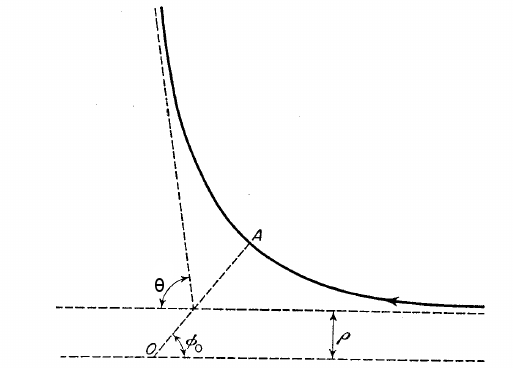
\includegraphics[scale=0.8]{Chapter1/sc.png}
    \caption{Diagram of scattering for a particle in a potential field\cite{landau}}
    \label{sc2}
\end{figure}
In a scattering of a beam of identical particles with velocity of $v$ , let $dN$ the number of particles scattered per unit of time through the angles $\theta$ and $\theta +d\theta$
The effective cross section is 
\begin{align}
    d\sigma=\frac{dN}{n}
\end{align}
n represents the number of particles passing in unit of time in a unit area of beam cross section. If $\rho$ is $\theta$ dependient, then the effective cross section is 
\begin{align}
    dN=2\phi \rho n d\rho \qquad d\sigma=2\phi \rho d\rho
\end{align}
rewriting $d\sigma$

\begin{align}
    d\sigma=2\phi \rho \left| \frac{d\rho}{d\theta} \right| d\theta
\end{align}
the derivative $\frac{d\rho}{d\theta}$ can be negative ,so it is necessary the modulus \cite{landau}. In a three dimension model, $d\sigma$ is related to the solid angle, instead of $d\theta$ , so the solid angle between the angles $\theta$ and $\theta+d\theta$ is
\begin{align}
    d\Omega=2\pi \sin{\theta}d\theta
\end{align}
thus, the cross section is 
\begin{align}
     d\sigma=   \frac{\rho(\theta)}{\sin{\theta}} \left| \frac{d\rho}{d\theta} \right| d\Omega
\end{align}
\begin{figure}[!htbp]
\centering
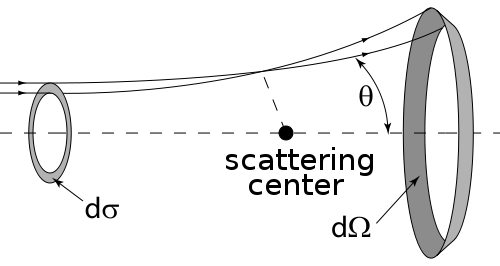
\includegraphics[scale=0.7]{Chapter1/cs1.png}
 \caption{Drawing of an idealized scattering process showing the differential solid angle $\Delta\Omega$ and the
scattering angle $\theta$ \cite{gross} }
\label{sc}
\end{figure}

let N be the number of events. In terms of of solid angle
\begin{align}
    dN=\text{L} d\sigma=\text{L} \frac{d\sigma}{d\Omega} d\Omega \qquad \frac{d\sigma}{d\Omega}=\frac{dN}{\text{L}d\Omega}
\end{align}
For a collision of two particles that produce many particles, the cross section is given by 
\begin{align}\label{sc3}
\sigma=\frac{S\hbar^2 }{4\sqrt{(p_1 \cdot p_2)^2 -(m_1 m_2 c^2)^2} }\int \left| M \right|^2 (2\pi)^4 \delta^4(p_1-p_2-...p_n)\times \prod_{j=2}^n 2\pi \delta (p_j^2-m_j^2 c^2)\theta (p_j^0)\frac{d^4 p_j}{(2\pi)^4}
\end{align} 
the structure of the equation \ref{sc3} is similar to the equation \ref{dm}\cite{griff}.\\

Experimentally
\begin{align}
d\sigma=\frac{\text{number of particles scattered into solid angle} \Delta\Omega}{\text{(number of particles incident)(scattering centers/area)}}
\end{align}